
\begin{question}
Consider the polynomial function below.

\[f(x)=3 x^{3} + 7 x + 9\]

Multiple choice: describe the end behavior.
\begin{answerlist}
  \item Down-down: when \(x\to -\infty\) then \(f(x)\to -\infty\) and when
\(x\to \infty\) then \(f(x)\to -\infty\).
  \item Up-down: when \(x\to -\infty\) then \(f(x)\to \infty\) and when
\(x\to \infty\) then \(f(x)\to -\infty\).
  \item Down-up: when \(x\to -\infty\) then \(f(x)\to -\infty\) and when
\(x\to \infty\) then \(f(x)\to \infty\).
  \item Up-up: when \(x\to -\infty\) then \(f(x)\to \infty\) and when
\(x\to \infty\) then \(f(x)\to \infty\).
\end{answerlist}
\end{question}

\begin{solution}
The degree of the polynomial is 3, which is odd. The highest-degree
term's coefficient is positive.

Thus the end behavior is down-up: when \(x\to -\infty\) then
\(f(x)\to -\infty\) and when \(x\to \infty\) then \(f(x)\to \infty\).

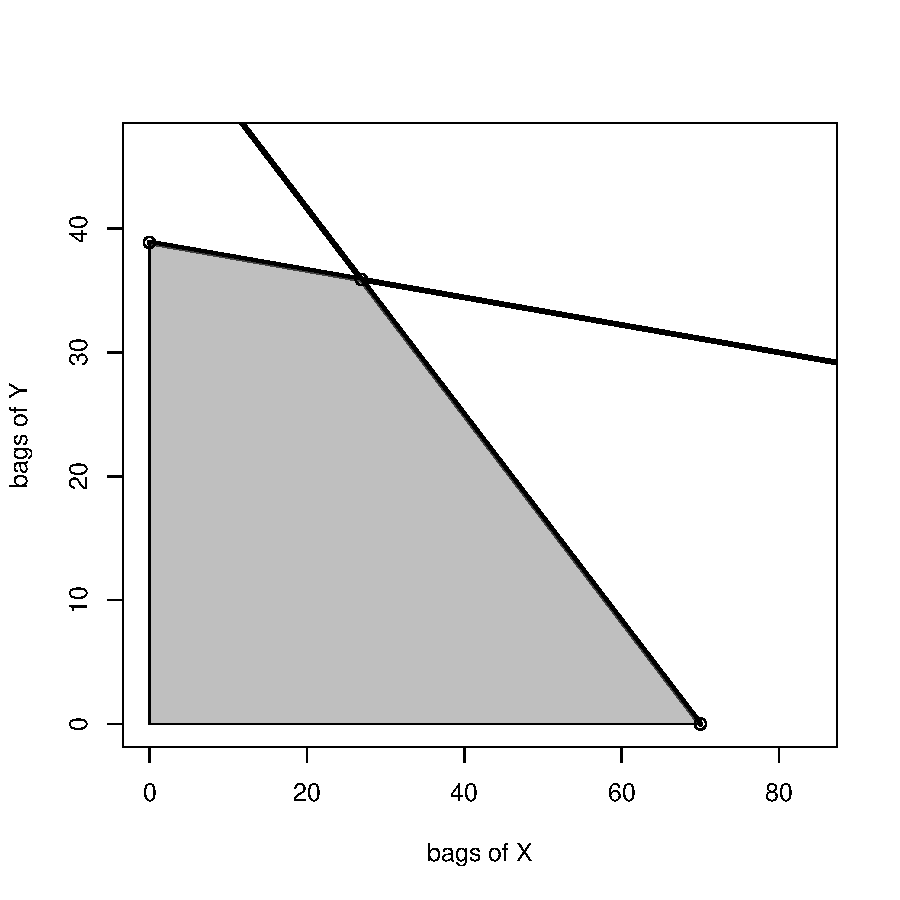
\includegraphics{unnamed-chunk-2-1.pdf} ~
\end{solution}

